\documentclass[../Main.tex]{subfiles}

\begin{document}

\section{Prototype 1}

The following document contains all the goals the first prototype of Steel Purge will reach at the end of the iteration. The goals will be very basic and must define the foundational structure of the game. Many of the current ideas written in the idea-document will be a part of the goals, so they will not be reiterated here.

\subsection{Gameplay}

The game is going to be a 2D action platformer in a tile-based world. The player is able to jump and walk like a normal platforming video game.

\subsubsection{Health}

The player has a total of 100 health. When the player takes damage, a timer will start which, when completed, starts a health regeneration process. The regeneration process is very slow and should only work out of combat. 

\subsubsection{Weapon mechanics}

Weapons can fire automatically by holding down a button or key. Weapons can shoot to the left, right or downwards. Firing downwards produces recoil which can propel the player upwards. Weapons can also be used to melee and they each have special damage numbers. They have special abilities which can be powered using unique fuels that can be crafted or found. 

\subsubsection{Weapons}

The following weapons from the ideas document will be implemented in Prototype 1:

\begin{itemize}
	\item Firewall
	\item Joule
	\item Neostar
\end{itemize}

\subsubsection{Movement mechanics}

The player will be able to slide on the ground to increase their speed shortly or to preserve their momentum if they managed to move fast initially. Using their weapon, the player can also aim downwards to fire which propels them a little higher each time they shoot. When the player walks for long enough, they will automatically start running slightly faster.

\subsubsection{Enemies}

 There will be two enemies and one boss at the end of the first level. When enemies are killed to hit, they drop scrap metal for the player. Enemies usually have a critical hit area on top of their head, meaning hits on this area will deal extra damage to them. 

\paragraph{}
The first enemy is the "XW Rush-Rogue", which is a small enemy with a high health pool. As soon as it sees the player, the enemy will rush towards the player. If the enemy hits the player, then it will explode dealing massive damage, almost killing the player. Since it has so much health and rushes towards the player, the enemy can receive massive critical hit damage that instantly kills it.

\paragraph{}
The second enemy is the "AR43 Executor". This enemy shoots three metal rods at a time and runs towards the player after each shooting interval. This enemy can also melee the player, which is why it runs towards them every interval.

\paragraph{}
The last enemy, which is a boss, is called the "TX9 Titan of Law". This enemy is a tall robot and has critical hit areas on its knees and head. It runs back and forth to stomp the player. Each iteration it smashes the ground and causes an earthquake dealing damage to the player. There should be platforming areas for the player to be able to reach the critical hit areas with a high risk and high reward. 

\subsubsection{Scrap}

Scrap is a material/currency which can be used to create/buy weapons and fuel. 

\subsubsection{Pickable items}

Steel Purge will have several items the player can pick up. For this prototype, there will only be scrap and weapons that can be picked up. The fuels must be crafted from scrap only.

\subsubsection{Checkpoints and crafting stations}

The checkpoints on the level will also serve as crafting stations. The player can craft respective fuels for their weapon they can craft using the scrap they collected from enemies

\subsection{User interface}

This section focuses on the user interface that will be present in the first prototype. There will be little descriptions of each interface and a figure with its overall design.

\subsubsection{Inventory/Start Menu}

\begin{figure}[H]
	\centering
	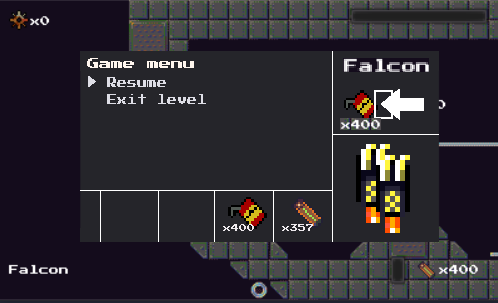
\includegraphics[width=\columnwidth]{Figures/InventoryUI.png}
	\caption{Inventory and start menu general design}
\end{figure}

\subsubsection{HUD}

\begin{figure}[H]
	\centering
	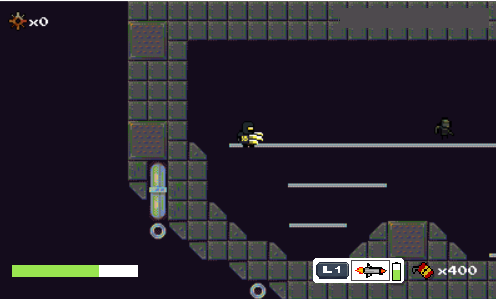
\includegraphics[width=\columnwidth]{Figures/HUD.png}
	\caption{HUD design (normally)}
\end{figure}


\begin{figure}[H]
	\centering
	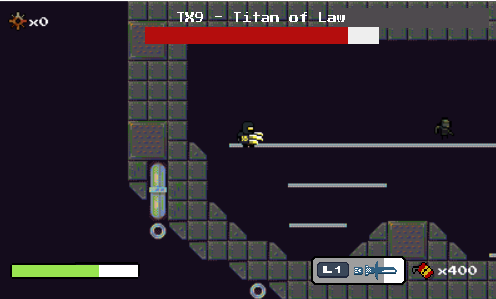
\includegraphics[width=\columnwidth]{Figures/HUDBoss.png}
	\caption{HUD design (active boss)}
\end{figure}

\subsubsection{Main Menu}

\begin{figure}[H]
	\centering
	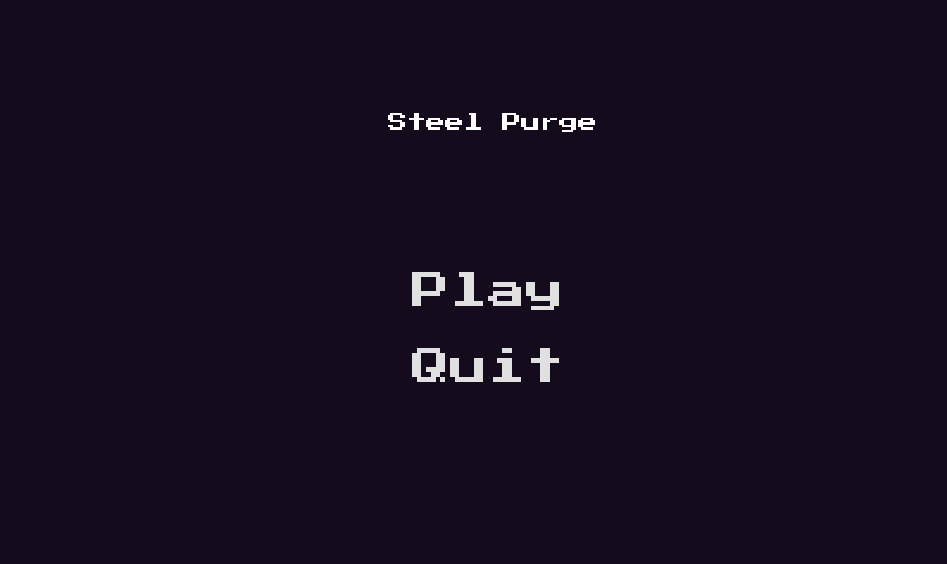
\includegraphics[width=\columnwidth]{Figures/StartMenu.png}
	\caption{Minimal viable main menu}
\end{figure}

\subsubsection{Shop Menu}

\subsection{Game Art}

The art in Steel Purge will currently be purely pixel art. For Prototype 1, the art will consist of somewhat altered free pixel art ripped from itch.io. There will also exist some custom art for the relevant areas, such as weapons. The following list will show the required art elements:

\textbf{Player}
\begin{itemize}
	\item Jump
	\item Walk
	\item Run
	\item Sliding
	\item Shooting alternating between each hand
	\item All animations above with different weapons equipped
\end{itemize}

\textbf{Weapon Sprites (General)}
\begin{itemize}
	\item Item icon on ground
	\item Icon in inventory
	\item Ordinance icon on HUD
\end{itemize}


\textbf{Firewall}
\begin{itemize}
	\item Dragons breath fire jet stream
\item Flares
\item Burn effect on enemies 
\end{itemize}

\textbf{Joule}
\begin{itemize}
	\item Bubble shield sprite
	\item Kinetic orb 
	\item Orb explosion
\end{itemize}

\textbf{Neostar}
\begin{itemize}
	\item Slam player animation
	\item Slam impact sprite
	\item Magnetic energy orbs
\end{itemize}

\textbf{Rush Rogue}
\begin{itemize}
	\item Patrolling
	\item Detecting player
	\item Rushing player
	\item Death
\end{itemize}

\textbf{Executor}
\begin{itemize}
	\item Shooting player
	\item Running towards player
	\item Death
\end{itemize}

\textbf{Titan of Law}
\begin{itemize}
	\item Running
	\item Slamming ground
	\item Death
\end{itemize}

% \textbf{}
% \begin{itemize}
% 	\item 
% \end{itemize}

\subsection{Music}

The main menu and first level will have their own respective music themes. 

\subsection{Sound Effects}

The following list will indicate all the game elements that require a sound effect\newline

\textbf{Player:}
\begin{itemize}
	\item Jumping
	\item Sliding
	\item Taking damage
	\item Dying
	\item Walking
	\item Sprint start
	\item Collecting scrap
	\item Collecting fuels (both Gasoline and Energy is different)
	\item Health regeneration start
	\item Health regeneration cancel
	\item Health regeneration fill per tick
	\item Health regeneration end after full health
\end{itemize}

\textbf{Enemies in general}
\begin{itemize}
	\item Taking damage (and dropping scrap)
	\item Taking critical damage
	\item Dying (make robotic collapse sound)
\end{itemize}

\textbf{Rush Rogue}
\begin{itemize}
	\item Detecting Player
	\item Rushing Player
	\item Exploding on player
\end{itemize}

\textbf{Executor}
\begin{itemize}
	\item Firing rods
	\item Walking towards player
\end{itemize}

\textbf{Titan of Law}
\begin{itemize}
	\item Ground slam
	\item Stomp Run
\end{itemize}

\textbf{Weapons}
\begin{itemize}
	\item When picked up (different for every weapon)
	\item Firing (different for every weapon)
	\item Ordinance used (different for every weapon)
	\item Ordinance ready
\end{itemize}

\textbf{Menus in general}
\begin{itemize}
	\item Button selection
	\item Button clicking
	\item Special button click (i.e, switching menu when pressed, crafting item in inventory)
\end{itemize}


\textbf{Inventory and Shop}
\begin{itemize}
	\item Open
	\item Close
\end{itemize}

\subsection{The first level}

\end{document}
